\subsection{Giới thiệu}
\textbf{IDS ( Intrusion Detection System – hệ thống phát hiện xâm nhập)} là một hệ thống giám sát lưu lượng mạng, có khả năng phát hiện các hoạt động khả nghi và cảnh báo cho hệ thống hoặc người quản trị mạng.
IDS phát hiện dựa trên các dấu hiệu đặc biệt về các nguy cơ đã biết hoặc dựa trên việc so sánh lưu lượng mạng hiện tại với baseline.
Trong đó baseline cho những hành vi bình thường được thiết lập bởi hồ sơ người dùng, máy chủ, hoặc hoạt động mạng trong quá trình học.
Sau khi quá trình học kết thúc, những phát hiện bất thường được tìm ra sau quá trình thăm dò của IDS bị chệch đi so với baseline này.
Phát hiện xâm nhập là một công việc khó khăn do sự phát triển nhanh chóng các của mạng lưới mạng, quá nhiều môi trường máy tính dẫn đến tính bất đồng bộ, nhiều giao thức mạng và sự phân loại đáng kể của các ứng dụng thông dụng và độc quyền. 
Hầu hết IDS sử dụng các dấu hiệu đặc biệt về nguy cơ xâm nhập đã biết( tương tự đối với cách mà các chương trình diệt virus hiện nay sử dụng để phát hiện và diệt virus), và sự khác biệt ứng xử của dấu hiệu xâm nhập so với những dấu hiệu đến từ người dùng thông thường.
\par
IDS thường được đặt ở nhiều vị trí trong hệ thống mạng, trong đó, vị trí phía sau Firewall được nhiều nhà quản trị tin dùng nhất. ở vị trí này, IDS có nhiệm vụ phân tích các gói tin đã được Firewall thông qua, xác định các dấu hiệu đã được định nghĩa mà Firewall không thể kiểm tra hoặc ngăn chặn. Từ các dấu hiệu này, IDS cung cấp thông tin và đưa ra các cảnh báo cho người quản trị viên.
\par
Với việc bảo vệ an toàn thông tin mạng ở một mức độ cao. 
Nhiều chuyên gia cho rằng IDS có giá trị giống như Firewall và VPN là ngăn ngừa các cuộc tấn công mà trong đó IDS cung cấp sự an toàn bằng cách trang bị cho bạn thông tin về các cuộc tấn công.
Chính vì điều này, IDS có thể đáp ứng nhu cầu về an toàn hệ thống bằng cách cảnh báo về khả năng có thể xảy ra của các cuộc tấn công và đôi khi bên cạnh các cảnh báo đúng thì chúng cũng mắc phải một số nhầm lẫn dần đến các cảnh báo chưa chính xác.
\subsection{Chức năng}
Nhìn chung, bản thân IDS không có khả năng tự động ngăn chặn các cuộc tấn công, tuy nhiên, các phiên bản hiện đại của IDS như IPS (sẽ được nhắc đến ở những chương sau) đã có thể thực hiện nhiều vai trò hơn và có thể ngăn chặn các cuộc tấn công khi nó xảy ra. 
Thực tế, IDS dường như chỉ thông báo cho chúng ta biết rằng mạng đang có dấu hiệu bị tấn công và đang ở trong giai đoạn nguy hiểm.
\par
Hệ thống phát hiện xâm nhập cho phép các tổ chức bảo vệ hệ thống mạng khỏi những đe dọa với việc gia tăng kết nối mạng và sự tin cậy của hệ thống thông tin, bổ sung cho những điểm yếu của hệ thống khác…
Sau đây là một vài lý do mà một hệ thống nên sử dụng IDS:
\begin{itemize}
\item Bảo vệ tính toàn vẹn dữ liệu, đảm bảo sự nhất quán của dữ liệu trong hệ thống. Các biện pháp đưa ra có khả năng ngăn chặn được sử thay đổi bất hợp pháp hoặc phá hoại dữ liệu.
\item Bảo vệ tính riêng tư, nghĩa là đảm bảo cho người sử dụng khai thác tài nguyên của hệ thống theo đúng chức năng nhiệm vụ đã được phân quyền, ngăn chặn được sự truy cập thong tin bất hợp pháp.
\item Bảo vệ tính bí mật, giữ cho thông tin không bị để lộ ra ngoài phạm vi cho phép.
\item Bảo vệ tính khả dụng, nghĩa là hệ thống luôn sẵn sàng thực hiện yêu cầu truy cập thông tin của người dùng hợp pháp.
\item Cung cấp thông tin về sự truy cập, đưa ra các chính sách đối phó, khôi phục, sửa chữa…
\end{itemize}
Về cơ bản, hệ thống IDS có thể giúp chúng ta ngăn ngừa các sự kiện tấn công trước khi nó xảy ra, cung cấp một số các giải pháp cho mạng và máy chủ, thậm chí cũng có thể hoạt động như một chuông báo động. 
Tuy nhiên chức năng chính của nó là thông báo cho người quản trị biết về các sự kiện có liên quan đến an ninh hệ thống đang sắp sửa xảy ra trong mạng và hệ thống mà người quản trị hiện đang kiểm soát.
\par
Thông thường, để phân loại IDS (IPS), người ta thường dựa vào đặc điểm của nguồn dữ liệu thu thập được. Trong trường hợp này, các hệ thống IDS được chia thành hai loại phổ biến như sau:
\begin{itemize}    
\item Host-Based IDS (HIDS): Sử dụng dữ liệu kiểm tra từ một máy trạm đơn để phát hiện xâm nhập.
\item Network-Based IDS (NIDS): Sử dụng dữ liệu trên toàn bộ lưu thông mạng, cùng với dữ liệu kiểm tra từ một hoặc một vài máy trạm để phát hiện xâm nhập.
\end{itemize}
\subsection{NIDS}
Hệ thống IDS dựa trên mạng sử dụng bộ dò và bộ cảm biến được cài đặt trên toàn mạng. Những bộ dò này theo dõi trên mạng với mục đích tìm kiếm những lưu lượng mạng khớp với những dấu hiệu được mô tả, định nghĩa từ trước. Những bộ cảm biến thu nhận và phân tích lưu lượng trong hệ thống thời gian thực. Khi nhận được mẫu lưu lượng hay dấu hiệu, bộ cảm biến gửi cảnh báo đến trạm quản trị và có thể được cấu hình nhằm tìm ra biện pháp ngăn chặn những xâm nhập xa hơn. NIDS là tập hợp nhiều cảm biến được cài đặt ở trên toàn mạng nhằm theo dõi những gói tin trong mạng, so sánh với mạng được định nghĩa để phát hiện đó là tấn công hay không.
\par
NIDS được đặt giữa hệ thống mạng bên trong và hệ thống mạng bên ngoài để giám sát toàn bộ lưu lượng vào ra. Có thể là một thiết bị phần cứng riêng biệt được thiết lập sẵn hay phần mềm cài đặt trên máy tinh, chủ yếu dùng để đo lưu lượng mạng được sử dụng.
\begin{figure}[!htbp]
    \centering
    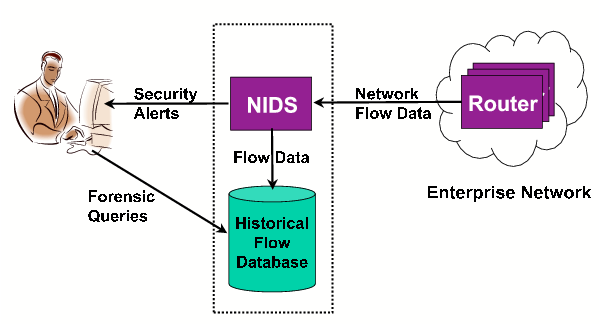
\includegraphics[scale=0.7]{nids}
    \caption{Luồng hoạt động của NIDS}
    \label{fig:x cubed graph}
\end{figure}
\FloatBarrier
NIDS giám sát toàn bộ mạng con của nó bằng cách lắng nghe tất cả các luồng dữ liệu trên mạng con đó. (Nó thay đổi chế độ hoạt động của card mạng NIC vào trong chế độ promisuous). Bình thường, một NIC hoạt động ở chế độ nonpromisuous nghĩa là nó chỉ nhận các gói tin mà có địa chỉ MAC khớp với địa chỉ của nó, các gói tin khác sẽ không nhận, hoặc không xử lý và bị loại bỏ.
Để giám sát tất cả các đường truyền trong mạng con, NIDS phải chấp nhận tất cả các gói tin và chuyển chúng tới ngăn xếp để xử lý. Do vậy nó sẽ phải cài đặt chế độ hoạt động cho card mạng là promisuous.
\newline
\newline
\textbf{Ưu điểm}
\begin{itemize}
    \item Chi phí triển khai thấp
    \item Phát hiện được các cuộc tấn công mà HIDS bỏ qua. 
    \newline Khác với HIDS, NIDS kiểm tra header của tất cả các gói tin vì thế hầu như không bỏ sót các dấu hiệu xuất phát từ đây.
    \item Khó xóa bỏ dấu vết (evidence)
    \item Phát hiện và đối phó kịp thời
    \item Có tính độc lập cao
\end{itemize}
\textbf{Nhược điểm}
\begin{itemize}
    \item Bị hạn chế với Switch
    \item Hạn chế về hiệu năng
    \item Tăng băng thông mạng
    \item Một hệ thống NIDS thường gặp khó khăn trong việc xử lý các cuộc tấn công trong một phiên được mã hóa
    \item Một hệ thống NIDS cũng gặp khó khăn khi phát hiện các cuộc tấn công mạng từ các gói tin phân mảnh
\end{itemize}
\subsection{HIDS}
Host-based IDS tìm kiếm dấu hiệu của xâm nhập trong một máy chủ cục bộ; thường sử dụng các cơ chế kiểm tra và phân tích các thông tin được lưu lại. 
Chủ yếu tìm kiếm các hoạt động bất thường như đăng nhập, truy cập tập tin không được cấp phép, bước leo thang các đặc quyền không được chấp nhận. 
Kiến trúc IDS này thường dựa trên các luật (rule-based) để phân tích các hoạt động. 
Ví dụ, đặc quyền của người sử dụng ở quyền bậc cao chỉ có thể thành công thông qua lệnh su-select user, như vậy những hành vi đăng nhập liên tục vào tài khoản root có thể được coi là một cuộc tấn công.
\newline
\newline
\textbf{Ưu điểm}
\begin{itemize}
    \item Xác định được kết quả của cuộc tấn công
    \item Khả năng giám sát các hoạt động cụ thể của hệ thống
    \item Phát hiện các hoạt động xâm nhập mà NIDS không phát hiện được: chẳng hạn kẻ tấn công sử dụng bàn phím xâm nhập vào một máy chủ sẽ không bị NIDS phát hiện.
    \item Không yêu cầu thêm phần cứng
\end{itemize}
\textbf{Nhược điểm}
\begin{itemize}
    \item Khó quản trị
    \item Nguồn thông tin phân tích không an toàn
    \item Hệ thống host-based khá đắt
    \item Chiếm tài nguyên hệ thống
\end{itemize}
